\documentclass[NET,english]{tumbeamer}

% If you load additional packages, do so in packages.sty as figures are build
% as standalone documents and you may want to have effect on them, too.

% Folder structure:
% .
% ├── beamermods.sty                  % depricated an will be removed soon
% ├── compile                         % remotely compile slides
% ├── figures                         % all figures go here
% │   └── schichtenmodelle_osi.tikz   % each .tikz or .tex is a target
% ├── include                         % create your document here
% │   ├── example.tex                 % example document
% │   └── slides.tex                  % make document wide changes here
% ├── lit.bib                         % literature
% ├── Makefile
% ├── moeptikz.sty                    % fancy networking symbols
% ├── packages.sty                    % load additional packages there
% ├── pics                            % binary pcitures go here
% ├── slides.tex                      % main document (may be more than one)
% ├── tumbeamer.cls
% ├── tumcolor.sty                    % TUM color definitions
% ├── tumcontact.sty                  % TUM headers and footers
% ├── tumlang.sty                     % TUM names and language settings
% └── tumlogo.sty                     % TUM logos

% Configure author, title, etc. here:
\documentclass[NET,english]{tumbeamer}

% If you load additional packages, do so in packages.sty as figures are build
% as standalone documents and you may want to have effect on them, too.

% Folder structure:
% .
% ├── beamermods.sty                  % depricated an will be removed soon
% ├── compile                         % remotely compile slides
% ├── figures                         % all figures go here
% │   └── schichtenmodelle_osi.tikz   % each .tikz or .tex is a target
% ├── include                         % create your document here
% │   ├── example.tex                 % example document
% │   └── slides.tex                  % make document wide changes here
% ├── lit.bib                         % literature
% ├── Makefile
% ├── moeptikz.sty                    % fancy networking symbols
% ├── packages.sty                    % load additional packages there
% ├── pics                            % binary pcitures go here
% ├── slides.tex                      % main document (may be more than one)
% ├── tumbeamer.cls
% ├── tumcolor.sty                    % TUM color definitions
% ├── tumcontact.sty                  % TUM headers and footers
% ├── tumlang.sty                     % TUM names and language settings
% └── tumlogo.sty                     % TUM logos

% Configure author, title, etc. here:
\documentclass[NET,english]{tumbeamer}

% If you load additional packages, do so in packages.sty as figures are build
% as standalone documents and you may want to have effect on them, too.

% Folder structure:
% .
% ├── beamermods.sty                  % depricated an will be removed soon
% ├── compile                         % remotely compile slides
% ├── figures                         % all figures go here
% │   └── schichtenmodelle_osi.tikz   % each .tikz or .tex is a target
% ├── include                         % create your document here
% │   ├── example.tex                 % example document
% │   └── slides.tex                  % make document wide changes here
% ├── lit.bib                         % literature
% ├── Makefile
% ├── moeptikz.sty                    % fancy networking symbols
% ├── packages.sty                    % load additional packages there
% ├── pics                            % binary pcitures go here
% ├── slides.tex                      % main document (may be more than one)
% ├── tumbeamer.cls
% ├── tumcolor.sty                    % TUM color definitions
% ├── tumcontact.sty                  % TUM headers and footers
% ├── tumlang.sty                     % TUM names and language settings
% └── tumlogo.sty                     % TUM logos

% Configure author, title, etc. here:
\documentclass[NET,english]{tumbeamer}

% If you load additional packages, do so in packages.sty as figures are build
% as standalone documents and you may want to have effect on them, too.

% Folder structure:
% .
% ├── beamermods.sty                  % depricated an will be removed soon
% ├── compile                         % remotely compile slides
% ├── figures                         % all figures go here
% │   └── schichtenmodelle_osi.tikz   % each .tikz or .tex is a target
% ├── include                         % create your document here
% │   ├── example.tex                 % example document
% │   └── slides.tex                  % make document wide changes here
% ├── lit.bib                         % literature
% ├── Makefile
% ├── moeptikz.sty                    % fancy networking symbols
% ├── packages.sty                    % load additional packages there
% ├── pics                            % binary pcitures go here
% ├── slides.tex                      % main document (may be more than one)
% ├── tumbeamer.cls
% ├── tumcolor.sty                    % TUM color definitions
% ├── tumcontact.sty                  % TUM headers and footers
% ├── tumlang.sty                     % TUM names and language settings
% └── tumlogo.sty                     % TUM logos

% Configure author, title, etc. here:
\input{include/slides}

\begin{document}

% For lecture mode, you may want to build one set of slides per chapter but
% with common page numbering. If so,
% 1) create a new .tex file for each chapter, e.g. slides_chapN.tex,
% 2) set the part counter to N-1 (assuming chapters start at 0), and
% 3) and name your chapter by using the \part{} command.
%\setcounter{part}{-1}
%\part{Organisatorisches und Einleitung}

% Include source files from ./include (or ./include/chapN).
%\input{include/example}

% Include markdown source from ./pandoc
%\input{pandoc/example}

\section{Why VPNs are Important}
\begin{frame}{Why VPNs are Important}
	\begin{itemize}
		\item Todays business is multi-national and international
		\item Many distributed sites that need to be interconnected
		\item Provide a secure channel for communication over insecure medium
		\item Other usecases: VM interconnects, cell tower backbones, firm intra-nets
	\end{itemize}
	
	=> Need for high throughput solutions
	
	Current state-of-the-art: $\ll$10 Gbit/s~\footnote{64 KB packets, no packet loss, hardware accelerated ciphers only}
\end{frame}

\begin{frame}{Focus: Site-to-Site VPN}
	\begin{figure}
		\centering
		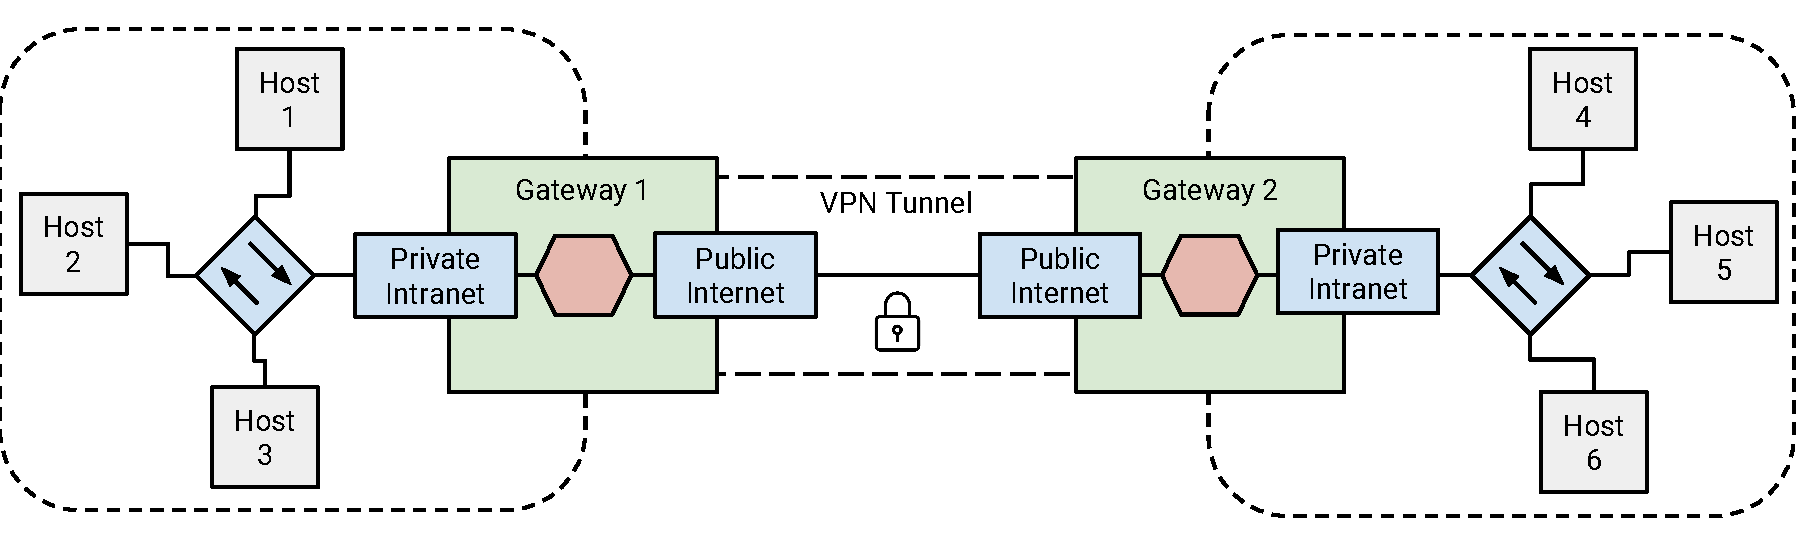
\includegraphics[width=1\linewidth]{figures/Site_to_Site_VPN}
		\caption{Overview of example Site-to-Site VPN setup}
		\label{fig:sitetositevpn}
	\end{figure}
	
	%Focus on Site-to-Site setups:
	\begin{itemize}
		\item Only two (or similar few) endpoints serving many hosts
		\item Very high bandwidth between them
	\end{itemize}
\end{frame}

\begin{frame}{Goals of this Thesis}
	\begin{itemize}
		\item Create benchmark criteria for Site-to-Site setups
		\item Evaluate performance of common implementations
		\item Develop a general performance model for VPNs
		\item Explore different approaches for performance improvements
	\end{itemize}
\end{frame}

\section{Overview of Existing Implementations}
\begin{frame}{Overview of Existing Implementations}
	\begin{itemize}
		\item OpenVPN
		\item IPsec
		\item WireGuard
	\end{itemize}

	Problems with them: Very slow under high load
\end{frame}

\begin{frame}
	\[ Insert graphs here \]
\end{frame}

\section{Improvements with MoonWire}
\begin{frame}{MoonWire}
	\begin{itemize}
		\item DPDK network stack to bypass slow kernel
		\item Lua for fast prototyping and interfacing with libraries (crypto)
	\end{itemize}
\end{frame}

\begin{frame}{MoonWire Graphs}
	 
	 [bytes/cycle graph of different ciphers]
	
	=> Cryptographic operations can become the bottleneck

	Hard to improve, correctness is more important
	
	Solution: work distribution to multiple cores
	
	WireGuard does this with Kernel worker tasks and a queue
	
	Lots of possible implementations
\end{frame}

\section{Case Study: Nonces in Symmetric Encryption}
\begin{frame}{Symmetric Encryption in a Nutshell}
	enc(Shared key + Nonce) = Encrypted message
	
	Correct nonce generation/handling is critical. Nonce reuse (under the same key) means K.O.
	
	Nonce generation depends on size. IETF ChaCha20 nonce is 96 bit (10 byte). 
	Too short to be randomly generated (birthday problem) => recommendation: counter++. Must be global over all threads/cores. Accessed for each packet => highly critical. Synchronization (mutex) and atomics are far too slow.
	
	[Timing graphs for atomics/mutex vs. mpps]
\end{frame}

\begin{frame}{Nonce Generation Tricks}

	\begin{itemize}
		\item Partition nonce space per worker: 8 bit worker\_id + 94 bit counter = 96 bit
		
		Worker$_{0}$: \textbf{0}123, \textbf{0}124, \textbf{0}125, ...
		
		Worker$_{1}$: \textbf{1}123, \textbf{1}124, \textbf{1}125, ...
		
		Beware of "overflows" into different worker partition
		
		\item Different cipher: XChaCha20 has 192 bit (24 byte) nonce
		
		Can be randomly generated safely. Each worker has own PRNG instance (seeded carefully) => Independent state, no sharing => fast
		
		Trade-off: messages get larger (by 10 bytes), incompatible with existing protocol
	\end{itemize}

	\pause
	Good news: Decryption is much easier. Message contains everything.
\end{frame}

\begin{frame}{Multi-core Scaling Opportunities}
	
	Source IP \& port identical over all packets => Simple RSS does not work
	
	
\end{frame}

\begin{frame}{Remaining Work}
	\begin{itemize}
		\item More benchmarking \& measurements
		\item Try more other performance improvements
		\begin{itemize}
			\item AVX512 cipher implementations \& CPU downclocking
			\item NUMA
		\end{itemize}
		\item Thesis writing
	\end{itemize}
\end{frame}

% Comment out if you do not want a bibliography
%\section{Bibliography}
%\begin{frame}[allowframebreaks]
%    \bibliographystyle{abbrv}
%    \setbeamertemplate{bibliography item}[text]
%    \footnotesize
%    \bibliography{lit}
%\end{frame}

\end{document}



\begin{document}

% For lecture mode, you may want to build one set of slides per chapter but
% with common page numbering. If so,
% 1) create a new .tex file for each chapter, e.g. slides_chapN.tex,
% 2) set the part counter to N-1 (assuming chapters start at 0), and
% 3) and name your chapter by using the \part{} command.
%\setcounter{part}{-1}
%\part{Organisatorisches und Einleitung}

% Include source files from ./include (or ./include/chapN).
%\documentclass[beamer,multi=true,preview]{standalone}
\usepackage{packages}

\standaloneenv{tikzpicture}

\let\myshipout\shipout
\begin{document}%
\let\shipout\myshipout

\begin{standaloneframe}[plain]%
\begin{tikzpicture}[>=latex]%
	\node[client] (client) at (0,0) {};
	\node[router] (router) at (2,0) {};
	\node[notebook] (notebook) at (4,0) {};

	\draw[line width=1pt] (client) to (router);
	\draw[line width=1pt] (router) to (notebook);
\end{tikzpicture}%
\end{standaloneframe}%
\end{document}%



% Include markdown source from ./pandoc
%\documentclass[beamer,multi=true,preview]{standalone}
\usepackage{packages}

\standaloneenv{tikzpicture}

\let\myshipout\shipout
\begin{document}%
\let\shipout\myshipout

\begin{standaloneframe}[plain]%
\begin{tikzpicture}[>=latex]%
	\node[client] (client) at (0,0) {};
	\node[router] (router) at (2,0) {};
	\node[notebook] (notebook) at (4,0) {};

	\draw[line width=1pt] (client) to (router);
	\draw[line width=1pt] (router) to (notebook);
\end{tikzpicture}%
\end{standaloneframe}%
\end{document}%



\section{Why VPNs are Important}
\begin{frame}{Why VPNs are Important}
	\begin{itemize}
		\item Todays business is multi-national and international
		\item Many distributed sites that need to be interconnected
		\item Provide a secure channel for communication over insecure medium
		\item Other usecases: VM interconnects, cell tower backbones, firm intra-nets
	\end{itemize}
	
	=> Need for high throughput solutions
	
	Current state-of-the-art: $\ll$10 Gbit/s~\footnote{64 KB packets, no packet loss, hardware accelerated ciphers only}
\end{frame}

\begin{frame}{Focus: Site-to-Site VPN}
	\begin{figure}
		\centering
		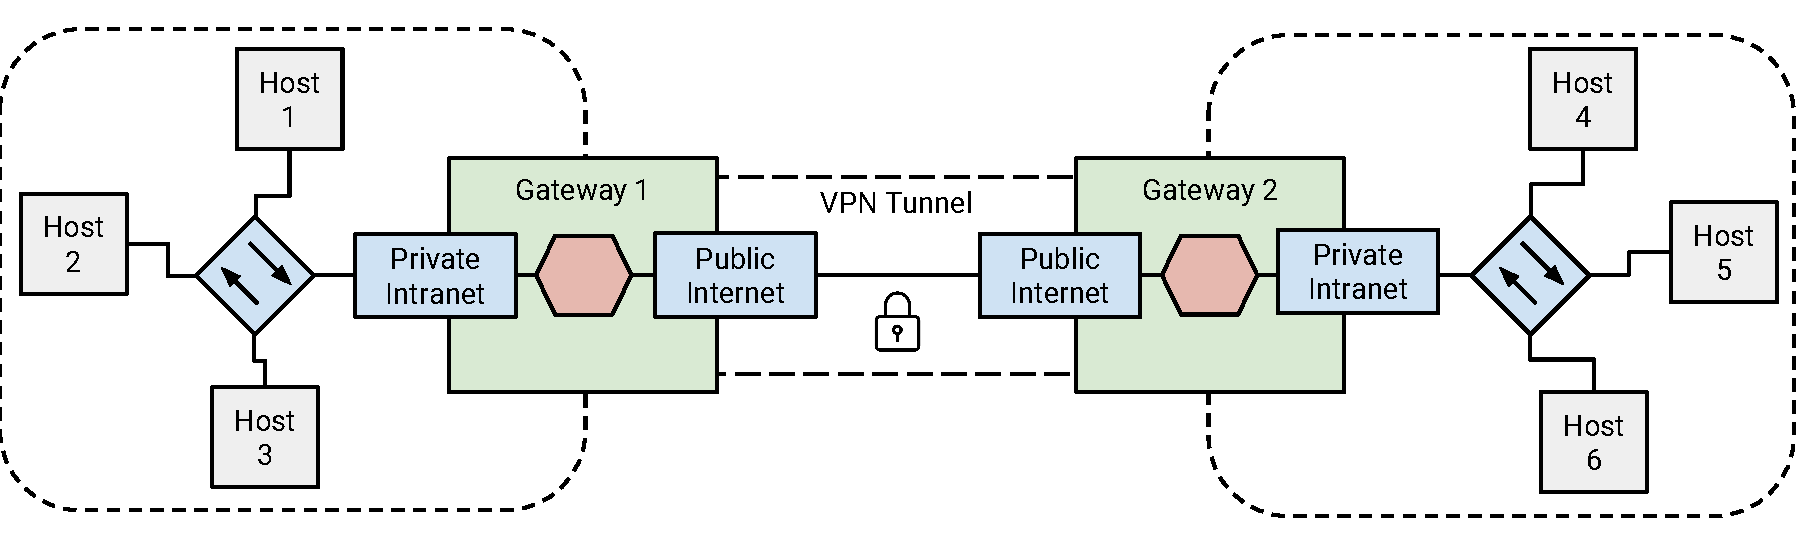
\includegraphics[width=1\linewidth]{figures/Site_to_Site_VPN}
		\caption{Overview of example Site-to-Site VPN setup}
		\label{fig:sitetositevpn}
	\end{figure}
	
	%Focus on Site-to-Site setups:
	\begin{itemize}
		\item Only two (or similar few) endpoints serving many hosts
		\item Very high bandwidth between them
	\end{itemize}
\end{frame}

\begin{frame}{Goals of this Thesis}
	\begin{itemize}
		\item Create benchmark criteria for Site-to-Site setups
		\item Evaluate performance of common implementations
		\item Develop a general performance model for VPNs
		\item Explore different approaches for performance improvements
	\end{itemize}
\end{frame}

\section{Overview of Existing Implementations}
\begin{frame}{Overview of Existing Implementations}
	\begin{itemize}
		\item OpenVPN
		\item IPsec
		\item WireGuard
	\end{itemize}

	Problems with them: Very slow under high load
\end{frame}

\begin{frame}
	\[ Insert graphs here \]
\end{frame}

\section{Improvements with MoonWire}
\begin{frame}{MoonWire}
	\begin{itemize}
		\item DPDK network stack to bypass slow kernel
		\item Lua for fast prototyping and interfacing with libraries (crypto)
	\end{itemize}
\end{frame}

\begin{frame}{MoonWire Graphs}
	 
	 [bytes/cycle graph of different ciphers]
	
	=> Cryptographic operations can become the bottleneck

	Hard to improve, correctness is more important
	
	Solution: work distribution to multiple cores
	
	WireGuard does this with Kernel worker tasks and a queue
	
	Lots of possible implementations
\end{frame}

\section{Case Study: Nonces in Symmetric Encryption}
\begin{frame}{Symmetric Encryption in a Nutshell}
	enc(Shared key + Nonce) = Encrypted message
	
	Correct nonce generation/handling is critical. Nonce reuse (under the same key) means K.O.
	
	Nonce generation depends on size. IETF ChaCha20 nonce is 96 bit (10 byte). 
	Too short to be randomly generated (birthday problem) => recommendation: counter++. Must be global over all threads/cores. Accessed for each packet => highly critical. Synchronization (mutex) and atomics are far too slow.
	
	[Timing graphs for atomics/mutex vs. mpps]
\end{frame}

\begin{frame}{Nonce Generation Tricks}

	\begin{itemize}
		\item Partition nonce space per worker: 8 bit worker\_id + 94 bit counter = 96 bit
		
		Worker$_{0}$: \textbf{0}123, \textbf{0}124, \textbf{0}125, ...
		
		Worker$_{1}$: \textbf{1}123, \textbf{1}124, \textbf{1}125, ...
		
		Beware of "overflows" into different worker partition
		
		\item Different cipher: XChaCha20 has 192 bit (24 byte) nonce
		
		Can be randomly generated safely. Each worker has own PRNG instance (seeded carefully) => Independent state, no sharing => fast
		
		Trade-off: messages get larger (by 10 bytes), incompatible with existing protocol
	\end{itemize}

	\pause
	Good news: Decryption is much easier. Message contains everything.
\end{frame}

\begin{frame}{Multi-core Scaling Opportunities}
	
	Source IP \& port identical over all packets => Simple RSS does not work
	
	
\end{frame}

\begin{frame}{Remaining Work}
	\begin{itemize}
		\item More benchmarking \& measurements
		\item Try more other performance improvements
		\begin{itemize}
			\item AVX512 cipher implementations \& CPU downclocking
			\item NUMA
		\end{itemize}
		\item Thesis writing
	\end{itemize}
\end{frame}

% Comment out if you do not want a bibliography
%\section{Bibliography}
%\begin{frame}[allowframebreaks]
%    \bibliographystyle{abbrv}
%    \setbeamertemplate{bibliography item}[text]
%    \footnotesize
%    \bibliography{lit}
%\end{frame}

\end{document}



\begin{document}

% For lecture mode, you may want to build one set of slides per chapter but
% with common page numbering. If so,
% 1) create a new .tex file for each chapter, e.g. slides_chapN.tex,
% 2) set the part counter to N-1 (assuming chapters start at 0), and
% 3) and name your chapter by using the \part{} command.
%\setcounter{part}{-1}
%\part{Organisatorisches und Einleitung}

% Include source files from ./include (or ./include/chapN).
%\documentclass[beamer,multi=true,preview]{standalone}
\usepackage{packages}

\standaloneenv{tikzpicture}

\let\myshipout\shipout
\begin{document}%
\let\shipout\myshipout

\begin{standaloneframe}[plain]%
\begin{tikzpicture}[>=latex]%
	\node[client] (client) at (0,0) {};
	\node[router] (router) at (2,0) {};
	\node[notebook] (notebook) at (4,0) {};

	\draw[line width=1pt] (client) to (router);
	\draw[line width=1pt] (router) to (notebook);
\end{tikzpicture}%
\end{standaloneframe}%
\end{document}%



% Include markdown source from ./pandoc
%\documentclass[beamer,multi=true,preview]{standalone}
\usepackage{packages}

\standaloneenv{tikzpicture}

\let\myshipout\shipout
\begin{document}%
\let\shipout\myshipout

\begin{standaloneframe}[plain]%
\begin{tikzpicture}[>=latex]%
	\node[client] (client) at (0,0) {};
	\node[router] (router) at (2,0) {};
	\node[notebook] (notebook) at (4,0) {};

	\draw[line width=1pt] (client) to (router);
	\draw[line width=1pt] (router) to (notebook);
\end{tikzpicture}%
\end{standaloneframe}%
\end{document}%



\section{Why VPNs are Important}
\begin{frame}{Why VPNs are Important}
	\begin{itemize}
		\item Todays business is multi-national and international
		\item Many distributed sites that need to be interconnected
		\item Provide a secure channel for communication over insecure medium
		\item Other usecases: VM interconnects, cell tower backbones, firm intra-nets
	\end{itemize}
	
	=> Need for high throughput solutions
	
	Current state-of-the-art: $\ll$10 Gbit/s~\footnote{64 KB packets, no packet loss, hardware accelerated ciphers only}
\end{frame}

\begin{frame}{Focus: Site-to-Site VPN}
	\begin{figure}
		\centering
		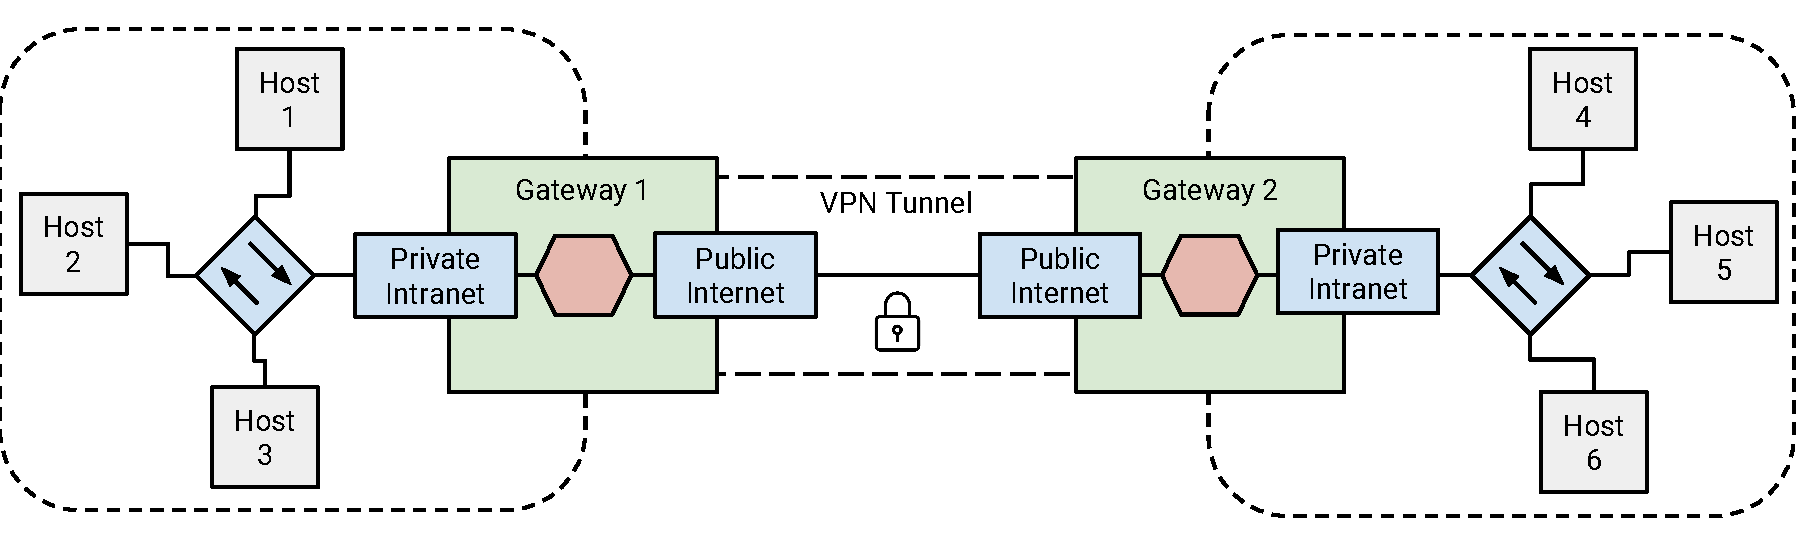
\includegraphics[width=1\linewidth]{figures/Site_to_Site_VPN}
		\caption{Overview of example Site-to-Site VPN setup}
		\label{fig:sitetositevpn}
	\end{figure}
	
	%Focus on Site-to-Site setups:
	\begin{itemize}
		\item Only two (or similar few) endpoints serving many hosts
		\item Very high bandwidth between them
	\end{itemize}
\end{frame}

\begin{frame}{Goals of this Thesis}
	\begin{itemize}
		\item Create benchmark criteria for Site-to-Site setups
		\item Evaluate performance of common implementations
		\item Develop a general performance model for VPNs
		\item Explore different approaches for performance improvements
	\end{itemize}
\end{frame}

\section{Overview of Existing Implementations}
\begin{frame}{Overview of Existing Implementations}
	\begin{itemize}
		\item OpenVPN
		\item IPsec
		\item WireGuard
	\end{itemize}

	Problems with them: Very slow under high load
\end{frame}

\begin{frame}
	\[ Insert graphs here \]
\end{frame}

\section{Improvements with MoonWire}
\begin{frame}{MoonWire}
	\begin{itemize}
		\item DPDK network stack to bypass slow kernel
		\item Lua for fast prototyping and interfacing with libraries (crypto)
	\end{itemize}
\end{frame}

\begin{frame}{MoonWire Graphs}
	 
	 [bytes/cycle graph of different ciphers]
	
	=> Cryptographic operations can become the bottleneck

	Hard to improve, correctness is more important
	
	Solution: work distribution to multiple cores
	
	WireGuard does this with Kernel worker tasks and a queue
	
	Lots of possible implementations
\end{frame}

\section{Case Study: Nonces in Symmetric Encryption}
\begin{frame}{Symmetric Encryption in a Nutshell}
	enc(Shared key + Nonce) = Encrypted message
	
	Correct nonce generation/handling is critical. Nonce reuse (under the same key) means K.O.
	
	Nonce generation depends on size. IETF ChaCha20 nonce is 96 bit (10 byte). 
	Too short to be randomly generated (birthday problem) => recommendation: counter++. Must be global over all threads/cores. Accessed for each packet => highly critical. Synchronization (mutex) and atomics are far too slow.
	
	[Timing graphs for atomics/mutex vs. mpps]
\end{frame}

\begin{frame}{Nonce Generation Tricks}

	\begin{itemize}
		\item Partition nonce space per worker: 8 bit worker\_id + 94 bit counter = 96 bit
		
		Worker$_{0}$: \textbf{0}123, \textbf{0}124, \textbf{0}125, ...
		
		Worker$_{1}$: \textbf{1}123, \textbf{1}124, \textbf{1}125, ...
		
		Beware of "overflows" into different worker partition
		
		\item Different cipher: XChaCha20 has 192 bit (24 byte) nonce
		
		Can be randomly generated safely. Each worker has own PRNG instance (seeded carefully) => Independent state, no sharing => fast
		
		Trade-off: messages get larger (by 10 bytes), incompatible with existing protocol
	\end{itemize}

	\pause
	Good news: Decryption is much easier. Message contains everything.
\end{frame}

\begin{frame}{Multi-core Scaling Opportunities}
	
	Source IP \& port identical over all packets => Simple RSS does not work
	
	
\end{frame}

\begin{frame}{Remaining Work}
	\begin{itemize}
		\item More benchmarking \& measurements
		\item Try more other performance improvements
		\begin{itemize}
			\item AVX512 cipher implementations \& CPU downclocking
			\item NUMA
		\end{itemize}
		\item Thesis writing
	\end{itemize}
\end{frame}

% Comment out if you do not want a bibliography
%\section{Bibliography}
%\begin{frame}[allowframebreaks]
%    \bibliographystyle{abbrv}
%    \setbeamertemplate{bibliography item}[text]
%    \footnotesize
%    \bibliography{lit}
%\end{frame}

\end{document}



\begin{document}

% For lecture mode, you may want to build one set of slides per chapter but
% with common page numbering. If so,
% 1) create a new .tex file for each chapter, e.g. slides_chapN.tex,
% 2) set the part counter to N-1 (assuming chapters start at 0), and
% 3) and name your chapter by using the \part{} command.
%\setcounter{part}{-1}
%\part{Organisatorisches und Einleitung}

% Include source files from ./include (or ./include/chapN).
%\documentclass[beamer,multi=true,preview]{standalone}
\usepackage{packages}

\standaloneenv{tikzpicture}

\let\myshipout\shipout
\begin{document}%
\let\shipout\myshipout

\begin{standaloneframe}[plain]%
\begin{tikzpicture}[>=latex]%
	\node[client] (client) at (0,0) {};
	\node[router] (router) at (2,0) {};
	\node[notebook] (notebook) at (4,0) {};

	\draw[line width=1pt] (client) to (router);
	\draw[line width=1pt] (router) to (notebook);
\end{tikzpicture}%
\end{standaloneframe}%
\end{document}%



% Include markdown source from ./pandoc
%\documentclass[beamer,multi=true,preview]{standalone}
\usepackage{packages}

\standaloneenv{tikzpicture}

\let\myshipout\shipout
\begin{document}%
\let\shipout\myshipout

\begin{standaloneframe}[plain]%
\begin{tikzpicture}[>=latex]%
	\node[client] (client) at (0,0) {};
	\node[router] (router) at (2,0) {};
	\node[notebook] (notebook) at (4,0) {};

	\draw[line width=1pt] (client) to (router);
	\draw[line width=1pt] (router) to (notebook);
\end{tikzpicture}%
\end{standaloneframe}%
\end{document}%



\section{Why VPNs are Important}
\begin{frame}{Why VPNs are Important}
	\begin{itemize}
		\item Todays business is multi-national and international
		\item Many distributed sites that need to be interconnected
		\item Provide a secure channel for communication over insecure medium
		\item Other usecases: VM interconnects, cell tower backbones, firm intra-nets
	\end{itemize}
	
	=> Need for high throughput solutions
	
	Current state-of-the-art: $\ll$10 Gbit/s~\footnote{64 KB packets, no packet loss, hardware accelerated ciphers only}
\end{frame}

\begin{frame}{Focus: Site-to-Site VPN}
	\begin{figure}
		\centering
		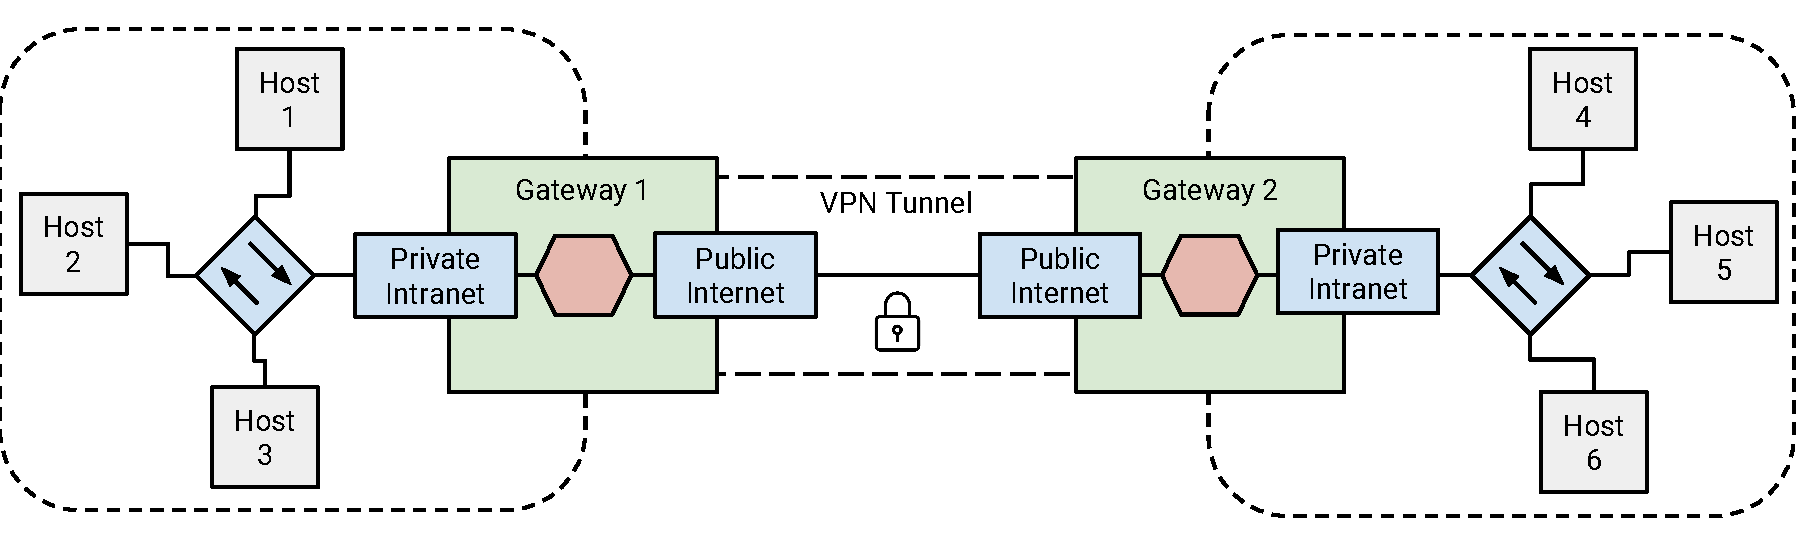
\includegraphics[width=1\linewidth]{figures/Site_to_Site_VPN}
		\caption{Overview of example Site-to-Site VPN setup}
		\label{fig:sitetositevpn}
	\end{figure}
	
	%Focus on Site-to-Site setups:
	\begin{itemize}
		\item Only two (or similar little) endpoints
		\item Very high bandwidth between them
	\end{itemize}
\end{frame}

\begin{frame}{Goals of this Thesis}
	\begin{itemize}
		\item Create benchmark criteria for Site-to-Site setups
		\item Evaluate performance of common implementations
		\item Develop a general performance model for VPNs
		\item Explore different approaches for performance improvements
	\end{itemize}
\end{frame}

\section{Overview of Existing Implementations}
\begin{frame}{Overview of Existing Implementations}
	\begin{itemize}
		\item OpenVPN
		\item IPsec
		\item WireGuard
	\end{itemize}

	Problems with them: Very slow under high load
\end{frame}

\begin{frame}
	\[ Insert graphs here \]
\end{frame}

\section{Improvements with MoonWire}
\begin{frame}{MoonWire}
	\begin{itemize}
		\item DPDK network stack to bypass slow kernel
		\item Lua for fast prototyping and interfacing with libraries (crypto)
	\end{itemize}
\end{frame}

\begin{frame}{MoonWire Graphs}
	 
	 [bytes/cycle graph of different ciphers]
	
	=> Cryptographic operations can become the bottleneck

	Hard to improve, correctness is more important
	
	Solution: work distribution to multiple cores
\end{frame}

\section{Case Study: Nonces in Symmetric Encryption}
\begin{frame}{Symmetric Encryption in a Nutshell}
	enc(Shared key + Nonce) = Encrypted message
	
	Correct nonce generation/handling is critical. Nonce reuse (under the same key) means K.O.
	
	Nonce generation depends on size. IETF ChaCha20 nonce is 96 bit (10 byte). 
	Too short to be randomly generated (birthday problem) => recommendation: counter++. Must be global over all threads/cores. Accessed for each packet => highly critical. Synchronization (mutex) and atomics are far too slow.
	
	[Timing graphs for atomics/mutex vs. mpps]
\end{frame}

\begin{frame}{Nonce Generation Tricks}

	\begin{itemize}
		\item Partition nonce space per worker: 8 bit worker\_id + 94 bit counter = 96 bit
		
		Worker$_{0}$: \textbf{0}123, \textbf{0}124, \textbf{0}125, ...
		
		Worker$_{1}$: \textbf{1}123, \textbf{1}124, \textbf{1}125, ...
		
		Beware of "overflows" into different worker partition
		
		\item Different cipher: XChaCha20 has 192 bit (24 byte) nonce
		
		Can be randomly generated safely. Each worker has own PRNG instance (seeded carefully) => Independent state, no sharing => fast
		
		Trade-off: messages get larger (by 10 bytes), incompatible with existing protocol
	\end{itemize}

	\pause
	Good news: Decryption is much easier. Message contains everything.
\end{frame}

\begin{frame}{Multi-core Scaling Opportunities}
	
	Source IP \& port identical over all packets => Simple RSS does not work
	
	
\end{frame}

\begin{frame}{Remaining Work}
	\begin{itemize}
		\item More benchmarking \& measurements
		\item Try more other performance improvements
		\begin{itemize}
			\item AVX512 cipher implementations \& CPU downclocking
			\item NUMA
		\end{itemize}
		\item Thesis writing
	\end{itemize}
\end{frame}

% Comment out if you do not want a bibliography
%\section{Bibliography}
%\begin{frame}[allowframebreaks]
%    \bibliographystyle{abbrv}
%    \setbeamertemplate{bibliography item}[text]
%    \footnotesize
%    \bibliography{lit}
%\end{frame}

\end{document}

